\documentclass{report}
\usepackage[utf8]{inputenc}

\title{N11: Plastic Number}
\author{Michael Hanna - 40075977 }
\date{}
\renewcommand{\baselinestretch}{1.15}

\usepackage{natbib}
\usepackage{graphicx}

\usepackage[final]{pdfpages}


\usepackage{fancyhdr}
\usepackage[margin=1in]{geometry}
\usepackage{pdfpages}
\renewcommand{\headrulewidth}{0.1pt}
\fancyhf{} 
\fancyhead[L]{\small Plastic Number} 
\fancyhead[C]{} 
\renewcommand{\headrulewidth}{0.1pt} 
\fancyfoot[C]{\thepage} 
\renewcommand{\footrulewidth}{0.1pt} 


\begin{document}
\maketitle
\tableofcontents

\chapter{Introduction}
\section{Value}
The Plastic number is known as the Plastic constant or Plastic ratio.\newline
\newline The value of the Plastic number is
\begin{eqnarray}
{\displaystyle \rho ={\sqrt[{3}]{\frac {9+{\sqrt {69}}}{18}}}+{\sqrt[{3}]{\frac {9-{\sqrt {69}}}{18}}}}
\end{eqnarray}
\newline Its decimal representation begin with 1.32471.\citep{pn}
\section{Uses}
It can be a way of partitioning a square into three rectangles.\newline
\newline A Rectangle of aspect ratio ${\rho}^2$  can be used for dissections of a square into similar rectangles \citep{pn}


\begin{figure}[h!]
\centering

\includegraphics[scale=0.5]{square}
\caption{Three partitions of a square into similar rectangles}
\label{fig:squares}
\end{figure}


\newpage
\newenvironment{qanda}{\setlength{\parindent}{0pt}}{\bigskip}
\newcommand{\Q}{\bigskip\bfseries Q: }
\newcommand{\A}{\par\textbf{A:} \normalfont}
 


\chapter{Interview}
\section{Questions \& Answers}
\begin{qanda}
 
\Q What are the operators do you use in a calculator?
\A I use all the operators.

\Q What do you dislike about a calculator?
\A I don't like writing long equations in a calculator.

\Q  How often do you use a calculator?
\A I use a calculator every day for my physics problems.

\Q  Do you like to use your mind to do the calculation or to use a calculator?
\A It depends, if the calculation is easy, then I would use my mind, however, if the number is more than 4 digits, then I would use a calculator.

\Q What constants do you want to have in a calculator?
\A I would like the calculator to have all possible constants since I like to have precise calculations for my experiments. for example: Pi,e,...

\Q Do you prefer a console or GUI calculator?
\A I would prefer to use MATLAB. 

\Q What are the functions do you wish to have in a calculator and didn't you find it yet?
\A Custom log base, Usually in calculators, you can only do ln and log, But log to the base 3 is not available.

\Q Have you ever had a bad experience with a calculator?
\A Accidentally, I pressed the erase button, so I needed to re-enter everything again.

\Q Do you like a calculator to plot a graph?
\A Yes

\Q do you prefer a real or soft calculator?
\A A real one, It's easy to carry it.

\Q Have you ever heard about the plastic number?
\A Yes.

\Q what is the application for that number?
\A it is used in Geometry; it can be used to partition a square into three rectangles.

\Q Finally, what are your recommendations?
\A I would recommend having a calculator with a large display, and it can plot a graph.

\section{Analysis}
Based on the conducted interview, a calculator is one of the most important assets for a mathematician as he/she can perform complex calculations.
Most of the mathematicians use a lot of irrational numbers and they preferred to have them all in the calculator, the user also preferred to have a way to save the equation if he accidentally press the clear button so he/she doesn't need to reenter it again and also the user prefers the calculator to have the option to plot a graph.


\end{qanda}
\newpage
\chapter{User Persona}
\begin{figure}[h!]
\centering
\includegraphics[scale=1, width=\paperwidth,angle=90]{Persona.png}
\label{fig:squares}
\end{figure}
\newpage
\chapter{Problem Domain}
\includepdf[pages=1]{ProblemDomain.pdf}
\newpage
\section{Description}
A calculator has 5 operators which are Add, Subtract, Multiply, Divide and Divide Square.
\subsection{User}
A user is a person who is using the calculator.
\subsection{Operator}
A user can use an operator to perform his calculation.\newline
\newline The Operator class is an interface class.
\subsection{OperatorValues}
The OperatorValues class shall be used to get the first and second value from the user.
\subsection{Operand}
Operand class shall be used to get all the irrational number. 
\subsection{PlasticNumber}
PlasticNumber is used to calculate the plastic number and also return the value of it. 
\subsection{DivideSquare}
The DivideSquare class shall implement the operator interface by dividing the square area by the plastic number and then display it.
\subsection{Add}
The Add class shall implement the operator interface by adding the two numbers and then display it.
\subsection{Subtract}
The Subtract class shall implement the operator interface by subtracting the two numbers and then display it.
\subsection{Multiply}
The Multiply class shall implement the operator interface by Multiply the two numbers and then display it.
\subsection{Divide}
The Divide class shall implement the operator interface by Dividing the two numbers and then display it.
\subsection{Display}
The Display class shall display the result after performing the calculation
\chapter{Activity Diagram}
\section{Description}
The user shall enter the first, second value and the operator that he wants to perform.\newline
\newline The next activity will be based on the operator that has been entered in the previous step.
\begin{itemize}
    \item If the user selects the "Add" function then the first and second values will be added
    \item If the user selects the "Subtract" function then the second will be subtracted from the first number.
    \item If the user selects the "Multiply" function then the first and second values will be Multiplied
    \item If the user selects the "Divide" function then the first will be divided by the second number
    \item If the user selects the "Divide Square" function then the first will be divided by plastic number.
\end{itemize}
Finally, after performing the calculation the results shall be displayed.

\includepdf[pages=1]{ActivityDiagram.pdf}
\newpage
\newpage
\chapter{Use Case Diagram}
\begin{figure}[h!]
\centering
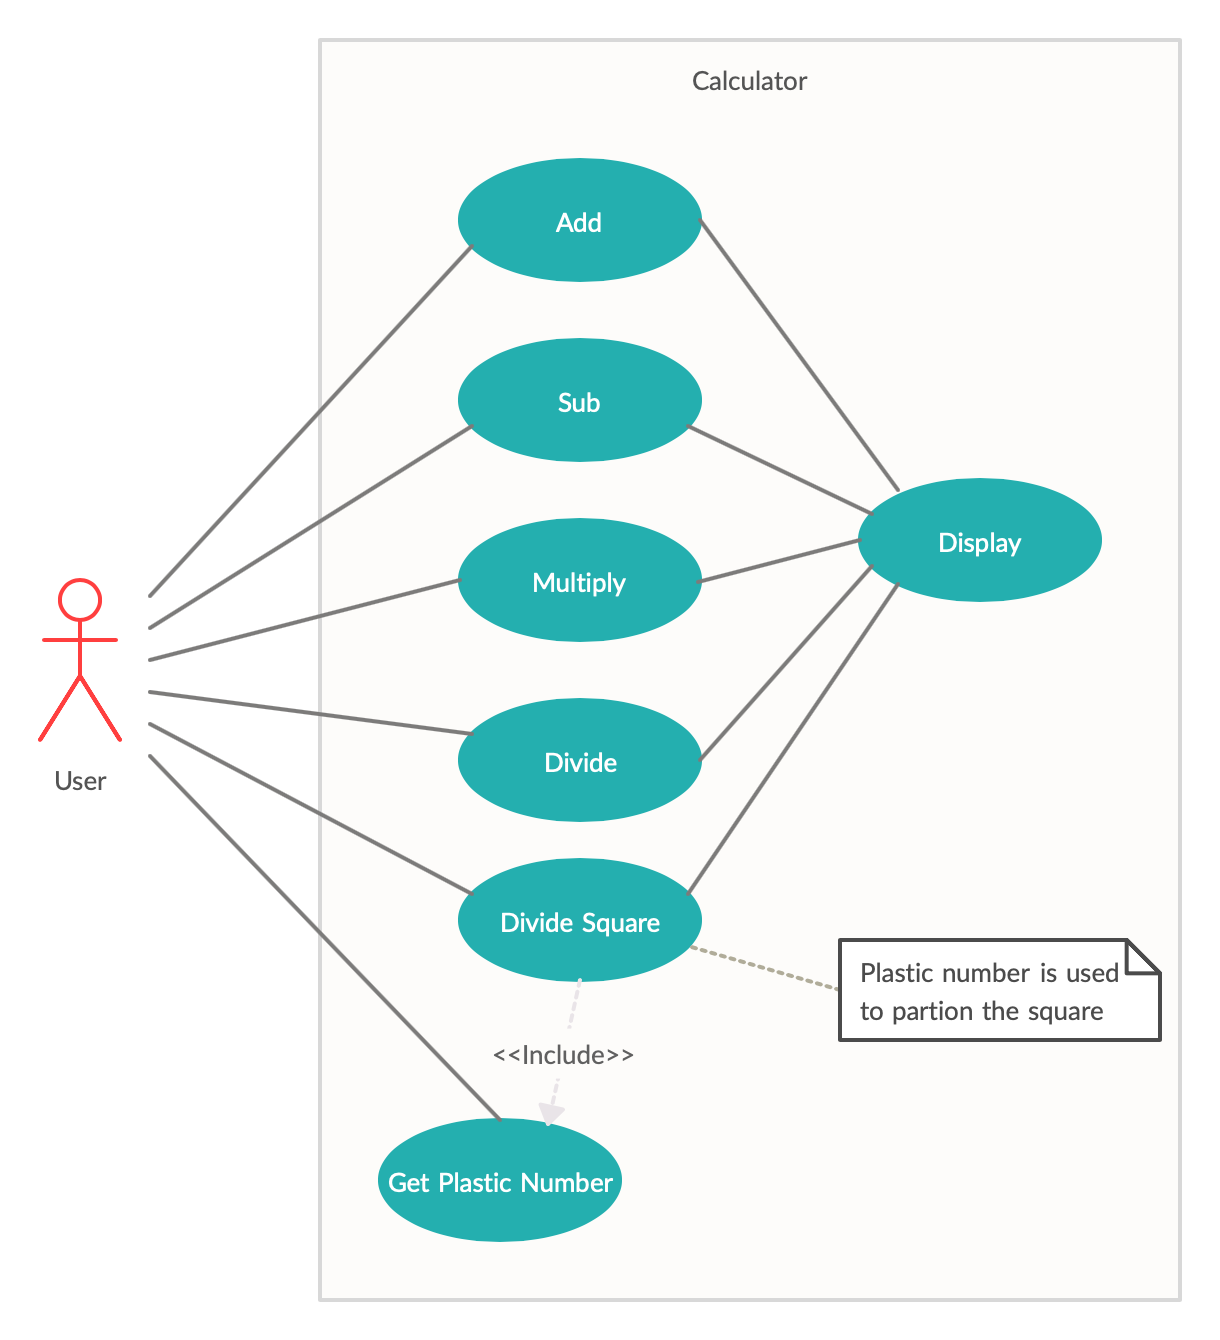
\includegraphics[scale=0.4]{UseCase.png}
\label{fig:UseCase}
\end{figure}
\section{Description}
The user has 6 use cases, each one has a unique goal as follow:
\begin{itemize}
    \item The goal of the "Add" Use case is to add the two numbers. 
    \item The goal of the "Sub" Use case is to subtract the two numbers. 
    \item The goal of the "Multiply" Use case is to Multiply the two numbers. 
    \item The goal of the "Divide" Use case is to divide the two numbers. 
    \item The goal of the "Divide Square" Use case is to partition the square.
    \item The goal of the "Get Plastic Number" Use case is to add two numbers. 
\end{itemize}
Finally, the goal of the "Display" use case is to display the results of the calculation.

\bibliographystyle{plain}
\bibliography{references}
\end{document}
